\subsection{代理模式(Proxy)}

\subsubsection{代理模式简介}

代理模式是一种设计模式,它提供了一种方法,通过使用一个中介对象来间接访问另一个对象,从而可以在不暴露目标对象的内部实现的情况下,对目标对象进行操作。

在代理模式中,代理对象充当目标对象的接口,从而可以控制对目标对象的访问。这种模式通常用于对目标对象进行限制、增强或保护性包装。

代理模式可以用于很多不同的应用场景,例如远程代理、虚拟代理、保护代理和缓存代理等。

在远程代理模式中,代理对象在客户端所在的机器上,而目标对象在远程服务器上,代理对象通过网络与目标对象进行交互。这种模式可以帮助客户端程序在本地访问远程对象,从而减少网络延迟。

在虚拟代理模式中,代理对象控制对目标对象的访问,并在客户端需要时才会创建目标对象。这种模式可以帮助减少系统开销,因为目标对象只在实际需要时才会创建。

在保护代理模式中,代理对象对目标对象进行保护性包装,只有当客户端满足特定条件时才能访问目标对象。这种模式可以用于实现访问控制,例如在需要身份验证的情况下。

在缓存代理模式中,代理对象缓存目标对象的结果,从而减少对目标对象的重复访问。这种模式可以帮助提高系统性能,因为通过减少对目标对象的访问,可以消除不必要的开销。

\subsubsection{代理模式在项目中的应用}

\begin{figure}[h]
  \centering
  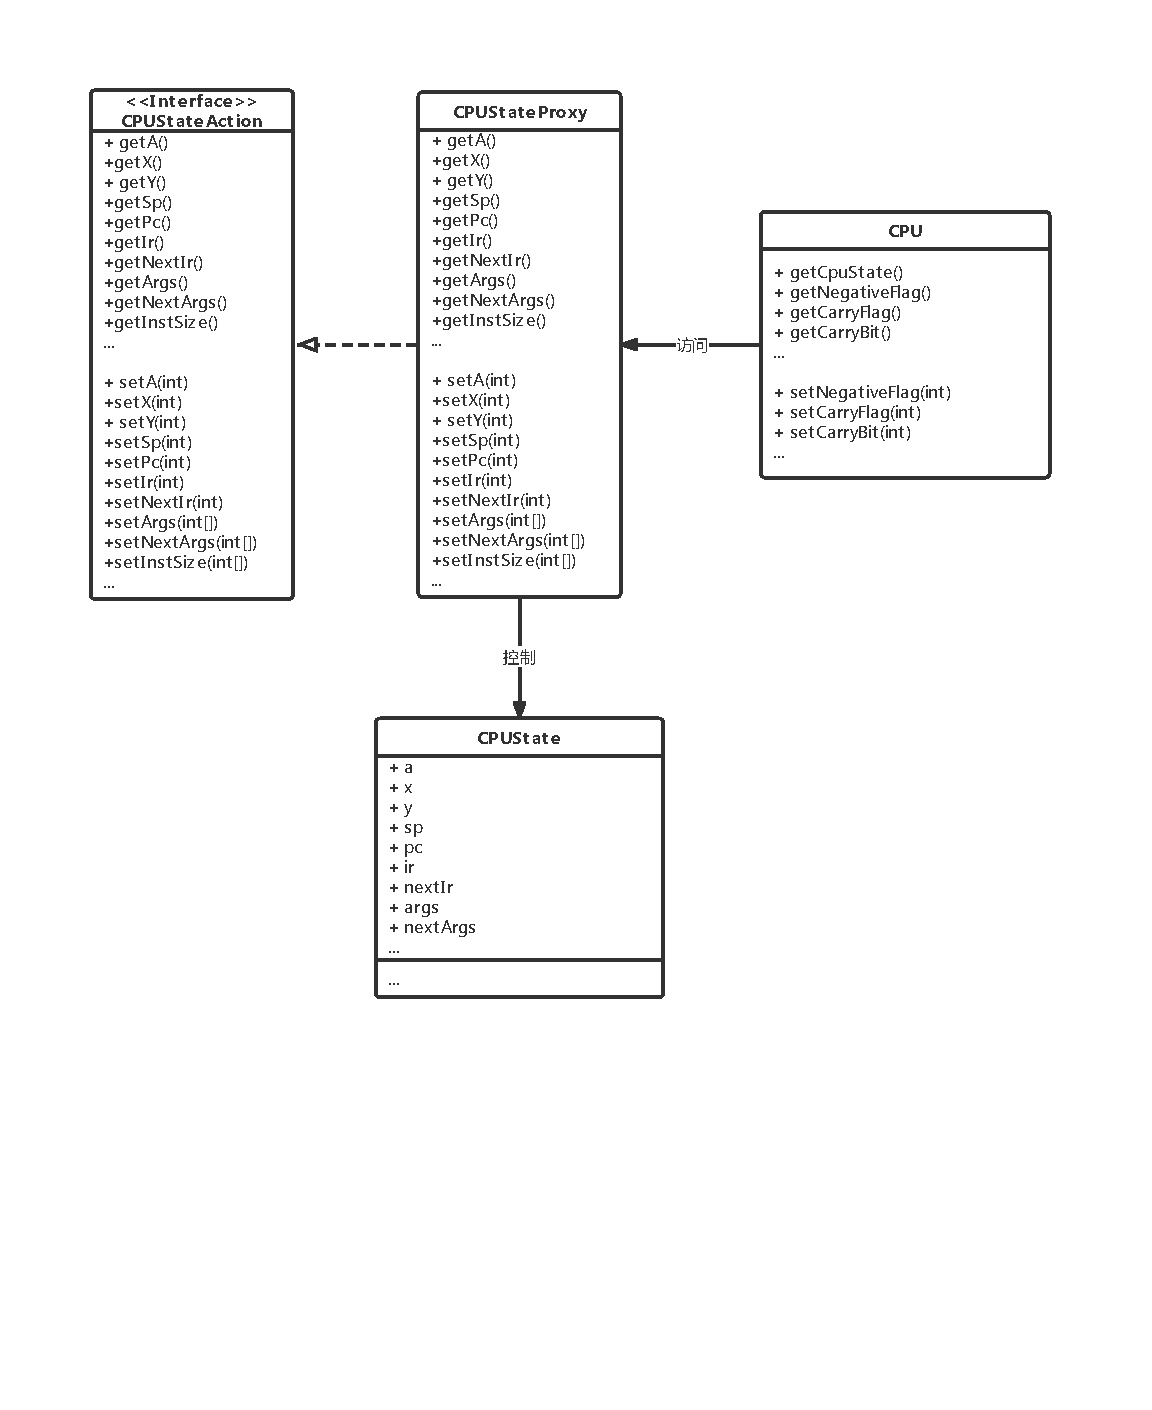
\includegraphics[width=0.9\textwidth]{figures/Proxy.pdf}
  \caption{代理模式在 Slow6502 中的类图}
\end{figure}

我们的项目中,使用代理模式包装对 CPU 内部状态的访问和修改。使用代理模式包装对 CPU 内部状态的访问和修改可以在不暴露CPU内部实现细节的情况下对其进行操作。这样的设计可以帮助保护 CPU 的实现,并且使得模拟器的其他部分只能通过代理对象来访问和修改 CPU 的状态,从而可以更好地控制对CPU的访问。

另外,使用代理模式还可以帮助模拟器更好地进行性能优化。例如,代理对象可以在内部缓存 CPU 的状态,从而减少对CPU的重复访问,从而提高模拟器的性能。
